\documentclass[ignorenonframetext, professionalfonts, hyperref={pdftex, unicode}]{beamer}
%\usepackage{beamerthemesplit}

\geometry{paperwidth=140mm,paperheight=105mm}

%Hack to specify beamer folder https://tex.stackexchange.com/questions/275600/beamer-themes-on-custom-folder
\makeatletter
  \def\beamer@calltheme#1#2#3{%
    \def\beamer@themelist{#2}
    \@for\beamer@themename:=\beamer@themelist\do
    {\usepackage[{#1}]{\beamer@themelocation/#3\beamer@themename}}}

  \def\usefolder#1{
    \def\beamer@themelocation{#1}
  }
  \def\beamer@themelocation{}
\makeatother
%Packages to be included

\usepackage{graphicx}



\graphicspath{{./branding/}}
\usefolder{./branding}
\usetheme{Promwad}
%\usecolortheme{wolverine}


\usepackage[russian]{babel}
\usepackage[utf8]{inputenc}
\usepackage[T1]{fontenc}

%\usepackage[orientation=landscape, size=custom, width=16, height=9, scale=0.5]{beamerposter}

\usepackage{textcomp}


\usepackage{ulem}

\usepackage{verbatim}

\usepackage{ucs}


\usepackage{listings}
\lstloadlanguages{bash}

\lstset{escapechar=`,
	extendedchars=false,
	language=sh,
	frame=single,
	tabsize=2, 
	columns=fullflexible, 
%	basicstyle=\scriptsize,
	keywordstyle=\color{blue}, 
	commentstyle=\itshape\color{brown},
%	identifierstyle=\ttfamily, 
	stringstyle=\mdseries\color{green}, 
	showstringspaces=false, 
	numbers=none, 
%	numberstyle=\tiny, 
	breaklines=true, 
	inputencoding=utf8,
	keepspaces=true,
	morekeywords={u\_short, u\_char, u\_long, in\_addr}
	}

\definecolor{darkgreen}{cmyk}{0.7, 0, 1, 0.5}

\lstdefinelanguage{diff}
{
    morekeywords={+, -},
    sensitive=false,
    morecomment=[l]{//},
    morecomment=[s]{/*}{*/},
    morecomment=[l][\color{darkgreen}]{+},
    morecomment=[l][\color{red}]{-},
    morestring=[b]",
}

\author[Promwad]{{\bf Promwad}}

%\institution[EPAM]{EPAM}
%\logo{\includegraphics[width=1cm]{logo.png}}

\AtBeginSection[]{%
  \begin{frame}<beamer>
    \frametitle{}
    \tableofcontents[
        sectionstyle=show/shaded, hideallsubsections ]
  \end{frame}
  \addtocounter{framenumber}{-1}% If you don't want them to affect the slide number
}

\AtBeginSubsection[]{%
  \begin{frame}<beamer>
    \frametitle{}
    \tableofcontents[
        sectionstyle=show/hide,
        subsectionstyle=show/shaded/hide, ]
  \end{frame}
  \addtocounter{framenumber}{-1}% If you don't want them to affect the slide number
}


\title{Ядро и драйверы устройств}

\begin{document}

\begin{frame}
  \frametitle{}
\end{frame}

\section{Анатомия ядра}

\begin{frame}
  \frametitle{Структура ядра}
  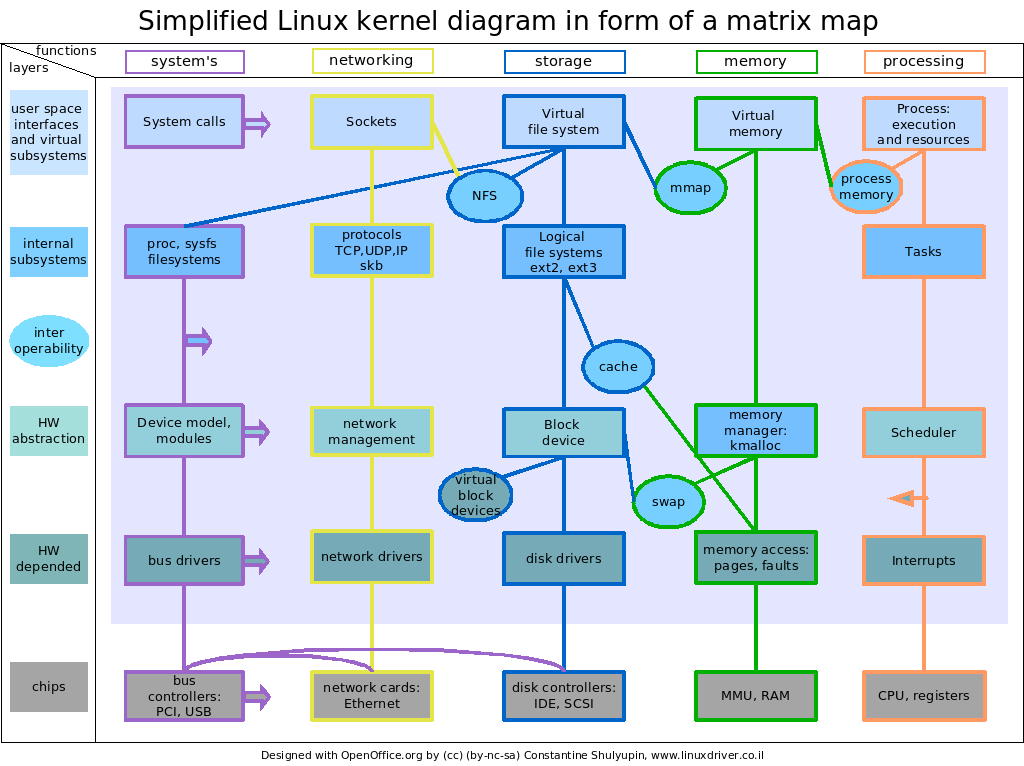
\includegraphics[width=9cm]{Linux_kernel_diagram.png}
\end{frame}

\section{Компиляция ядра}
\begin{frame}[fragile]
  \frametitle{Компиляция}
\begin{lstlisting}[language=bash]
make <board>_config
make menuconfig
make -j4
make INSTALL_MOD_PATH=<mod path> modules_install
make clean
make mrproper
\end{lstlisting}
\end{frame}

\begin{frame}[fragile]
  \frametitle{Кросс-компиляция}
\begin{lstlisting}[language=bash]
ARCH=arm CROSS_COMPILE=arm-linux-gnueabi- make <target>
\end{lstlisting}
\end{frame}
\section{Модули ядра}
\begin{frame}
  \frametitle{Модуль}
\textbf{Модуль} -- загружаемый объектный файл, связывающийся с ядром.
\vspace{1cm}
Функции модуля находятся в одном адресном пространстве с ядром и другими модулями (монолитное ядро).
\vspace{0.5cm}
\begin{center}
  \textbf{Зачем?}
\end{center}
\begin{itemize}
  \item Экономия памяти (не грузим ненужное)
  \item Можно скомпилировать сразу все
  \item Можно загружать разные модули в разных ситуациях
\end{itemize}
\end{frame}
\begin{frame}[fragile]
  \frametitle{Минимальный модуль ядра}
\begin{lstlisting}[language=C]
#include <linux/module.h>
#include <linux/kernel.h>
MODULE_LICENSE("Dual BSD/GPL");
MODULE_AUTHOR("John Doe");
MODULE_DESCRIPTION("Hello world");
MODULE_VERSION("0.1");
int __init hello_init(void){
    printk(KERN_ALERT "Hello, world!\n");
      return 0;
}
void __exit hello_exit(void){
        printk(KERN_ALERT "Goodbye, world -- exiting\n");
}
module_init(hello_init);
module_exit(hello_exit);
\end{lstlisting}
\end{frame}

\begin{frame}[fragile]
  \frametitle{Сборка модуля: out of tree}
\begin{lstlisting}[language=make]
ifneq ($(KERNELRELEASE),)
obj-m := hello.o
else
KDIR := ../linux
all:
        $(MAKE) -C $(KDIR) M=$$PWD modules
endif
\end{lstlisting}
\end{frame}

\begin{frame}[fragile]
  \frametitle{Сборка модуля: out of tree}
\begin{lstlisting}[language=bash]
ARCH=arm CROSS_COMPILE=arm-linux-gnueabi- make
\end{lstlisting}
\end{frame}

\begin{frame}
  \frametitle{Добавление модуля в инфраструктуру ядра}
  \begin{itemize}
    \item Добавить С файл модуля в подобающую по логике директорию
    \item Добавить описание модуля к Kconfig в директории
    \item Добавить \texttt{obj-\$\{CONFIG\_MODULE\_NAME\}} к Makefile в директории 
  \end{itemize}
\end{frame}

\begin{frame}[fragile]
  \frametitle{Загрузка и выгрузка модуля}
\begin{lstlisting}[language=bash]
insmod ./hello.ko # Наиболее непосредственная команда
lsmod | grep hello
rmmod hello
# Более правильно
modprobe hello # Разрешает зависимости модулей
cat /proc/modules
\end{lstlisting}

\end{frame}

\begin{frame}
  \frametitle{Что происходит при insmod}
  \begin{itemize}
    \item \textbf{user} 
      системный вызов \texttt{init\_module} копирует код модуля в ядро
    \item \textbf{kernel}
      \texttt{sys\_init\_module}
      \begin{itemize}
        \item Добавление модуля в связный список
        \item Выделение памяти для модуля, копирование кода в эту память
        \item Проверка (архитектура, исправность файла)
        \item Oкончательное выделение памяти
        \item Разрешение символов
        \item Вызов инициализации модуля, etc.
      \end{itemize}
  \end{itemize}
\end{frame}

\begin{frame}
  \frametitle{Выгрузка модуля}
  \begin{itemize}
    \item Системный вызов \texttt{delete\_module}
    \item Внутриядерный вызов \texttt{sys\_delete\_module}
      \begin{itemize}
        \item Проверяет, что модуль не используется другими модулями
        \item Проверяте, что модуль не используется процессами
        \item Вызывает процедуру деинициализации модуля
        \item Удаляет код модуля из памяти
      \end{itemize}
  \end{itemize}
\end{frame}

\begin{frame}[fragile]
  \frametitle{Передача параметров}
\begin{center}
  Userspace
\end{center}
\begin{lstlisting}[language=bash]
modprobe hello whom="world"
insmod hello.ko whom="world"
\end{lstlisting}
\end{frame}

\begin{frame}[fragile]
  \frametitle{Передача параметров}
\begin{center}
  Код модуля 
\end{center}
\begin{lstlisting}[language=C]
static char* whom="world";
module_param(whom,charp,0);
MODULE_PARM_DESC(whom,"Who to greet, default value -- \"world\"");
...
printk(KERN_ALERT "Hello, %s\n",whom);
\end{lstlisting}
\end{frame}

\begin{frame}
  \frametitle{Модули ядра vs userspace}
  \begin{itemize}
    \item Нет стандартной библиотеки (линковка только внутри ядра)
    \item Нет вещественных чисел (floating point)
    \item Маленький стек (может быть 4096 байт)
    \item Никто не освободит ресурсы за тебя
    \item Segmentation fault=все умерли
  \end{itemize}
\end{frame}

\section{Драйверы устройств}
\subsection{Классификация драйверов}
\begin{frame}
  \frametitle{Классификация модулей драйверов co стороны пользователя}
  \begin{itemize}
    \item Символьные устройства
    \item Блочные устройства
    \item Сетевые устройства
    \item Абстрактные устройства (драйверы шин, адаптеры)
  \end{itemize}
\end{frame}
\begin{frame}
  \frametitle{Классификация драйверов со стороны hardware}
  \begin{itemize}
    \item Драйверы шин с авторегистрацией
      \begin{itemize}
        \item USB драйверы
        \item PCI драйверы
      \end{itemize}
    \item Драйверы платформенных шин
      \begin{itemize}
        \item I$^2$C
        \item SPI
        \item UART
        \item ...
      \end{itemize}
  \end{itemize}
\end{frame}
\subsection{Символьные устройства}
\begin{frame}[fragile]
  \frametitle{Типичное использование символьного устройства}
\begin{lstlisting}[language=C]
int main(int argc, char **argv){
  int f,n;
  char rnd[100];
  f=open("/dev/urandom",O_RDONLY);
  n = read(f,&rnd,sizeof(rnd));
  close(f);
  return(0);
}
\end{lstlisting}
\end{frame}
\begin{frame}[fragile]
  \frametitle{Что реализует драйвер символьного устройства}
\begin{lstlisting}[language=C]
struct file_operations my_fops = {
  .owner = THIS_MODULE,
  .read = my_read_op,
  .write = my_write_op,
  .open = my_open_op,
  .release = my_release_op,
  .ioctl_unlocked = my_ioctl_op,
}
\end{lstlisting}
\end{frame}
\begin{frame}[fragile]
  \frametitle{Что реализует драйвер символьного устройства}
\begin{lstlisting}[language=C]
#include <linux/fs.h>
struct file_operations my_fops =...
static int __init chrdev_init(void){
    major = register_chrdev(0,"mychrdrv",&my_fops);
}
static int __exit chrdev_exit(void){
  unregister_chrdev(major,"mychrdrv");
}
module_init(chrdev_init);
...
\end{lstlisting}
\end{frame}

\begin{frame}[fragile]
  \frametitle{Более новый подход}
\begin{lstlisting}[language=C]
struct mydev_dev {
  /*dev data
  ...
  */
  struct cdev *cdev;
}
\end{lstlisting}
\end{frame}

\begin{frame}[fragile]
  \frametitle{Более новый подход}
\begin{lstlisting}[language=C]
static int __init mydev_init(void){
  dev_t mydev;
  int ret;
  ret = alloc_chrdev_region(&mydev,0,MAX_DEVS,"my_dev");
  if(ret) return ret;
  struct mydev_dev *dev = kzalloc(sizeof(),GFP_KERNEL);
  if(!mydev_dev) goto cleanup_alloc;
  cdev_init(&dev->cdev,&mydev_fops);
  ret=cdev_add(&dev->cdev,mydev,1);
  if(ret) goto cleanup_dev;
  return 0;
cleanup...:
return ret;
}
\end{lstlisting}
\end{frame}

\begin{frame}[fragile]
  \frametitle{Некоторые операции:open}
\begin{lstlisting}[language=C]
static mydev_open(struct inode *inode, struct file *filp){
  struct cdev *cdev = inode->i_cdev;
  filp->private_data=container_of(cdev,struct mydev_dev,cdev);
  /* initialize per file data
    ...
   */
 }
\end{lstlisting}
\end{frame}

\begin{frame}[fragile]
  \frametitle{Некоторые операции:read}
\begin{lstlisting}[language=C]
static mydev_read(struct file *file, char __user *buf, size_t count, loff_t *ppos){
  /*
  ...
  */
  copy_to_user(buf,data,size);
  read_count +=size;
  ...
  return read_count;
 }
\end{lstlisting}
\end{frame}
\begin{frame}[fragile]
  \frametitle{Некоторые операции:ioctl}
\begin{lstlisting}[language=C]
 static mydev_ioctl(struct inode *inode, struct file *file, unsigned int cmd, unsigned long arg){
   /*Check access */
   switch(cmd){
     ...
   }
 }
\end{lstlisting}
\end{frame}
\begin{frame}[fragile]
  \frametitle{Пример ioctl}
\begin{lstlisting}[language=C]
int main(int argc, char **argv){
  int fd = open("/dev/mydevice",O_RDWRITE);
  struct ioctl_arg {
    int field1;
    int field2;
  } my_arg;
  ioctl(fd,MY_DEV_COMMAND,&my_arg);
  close(fd);
}
\end{lstlisting}
\end{frame}

\begin{frame}[fragile]
  \frametitle{Современные драйверы устройств}
  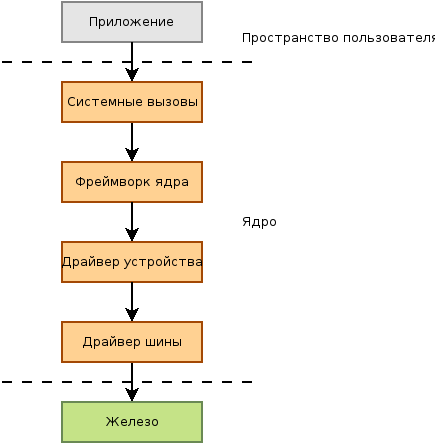
\includegraphics[width=7cm]{driver-architecture2.png}
\end{frame}  


\begin{frame}[fragile]
  \frametitle{Скелет драйвера платформенного устройства}
\begin{lstlisting}[language=C]
/* структура представляющая драйвер*/
static struct i2c_driver myi2cdev_driver = {
  .driver = {
    .name = "myi2cdev",
    .of_match_table = of_match_ptr(myi2cdev_of_match),
    .owner = THIS_MODULE,
  },
  .id_table = myi2cdev_id_table,
  .probe = myi2cdev_probe,
  .remove = myi2cdev_remove,
};

module_i2c_driver(myi2cdev_driver);
MODULE_AUTHOR("John Doe");
...
\end{lstlisting}
\end{frame}

\begin{frame}[fragile]
  \frametitle{Скелет драйвера платформенного устройства}
\begin{lstlisting}[language=C]
/*Devicetree related*/
#ifdef CONFIG_OF
static const struct of_device_id myi2cdev_of_match[] = {
  {.compatible = "hmc,myi2cdev83"},
};
#endif

static const struct i2c_device_id myi2cdev_id_table[] = {
  { "myi2cdev83",0},
  {},
};
MODULE_DEVICE_TABLE(i2c,myi2cdev_id_table);
\end{lstlisting}
\end{frame}

\begin{frame}[fragile]
  \frametitle{Скелет драйвера платформенного устройства}
\begin{lstlisting}[language=C]
static int myi2cdev_probe(struct i2c_client *client, const struct i2c_device_id *id){
  struct xxxclass_dev *xxxdev;
  struct xxxdev_data *data;
  if(!i2c_check_functionality(client->adapter,I2C_FUNC_SMBUS_WRITE_BYTE|..)
     return -EOPNOTSUPP;
  xxxdev = devm_xxx_device_alloc(&client->dev,sizeof(*data));
  if(!xxxdev)
     return -ENOMEM;
  /*init device*/
}

static int myi2cdev_remove(struct i2c_client *client){
}
\end{lstlisting}
\end{frame}

\subsection{sysfs}
\begin{frame}
  \frametitle{Sysfs}
\end{frame}
\subsection{Отладка}
\begin{frame}
  \frametitle{Способы отладки ядра}
  \begin{itemize}
    \item \texttt{printk} 
      \begin{itemize}
          \item CONFIG\_DEBUG
          \item CONFIG\_DYNAMIC\_DEBUG
      \end{itemize}
    \item CONFIG\_DEBUG\_FS
    \item qemu as gdb server
    \item kgdb
  \end{itemize}
\end{frame}

\section{Заключение}
\begin{frame}
  \frametitle{Литература}
  \begin{itemize}
    \item  Embedded Linux system design and development  P. Raghavan, Amol Lad, Sriram Neelakandan. (Разработка и внедрение системы на встраиваемом Linux)
    \item Mastering Embedded Linux Programming. Chris Simmonds (Крис Симмондс: Встраиваемые системы на основе Linux)
    \item Linux Device Drivers, 3rd edition. Corbet, Rubini, Kroah-Hartman 
    \item \url{https://free-electrons.com/training/}
  \end{itemize}
\end{frame}

\begin{frame}
  \frametitle{Ссылка для скачивания слайдов}
  \begin{center}
    \url{https://yadi.sk/d/uqJmLeCL3QkahA}
  \end{center}
\end{frame}

\end{document}
